\section{Descriptive analysis} 

\subsection{a)}
The variables included in the data set are: height, weight, gender, urbanity and fast food eaten in a year. Some of them are strictly quantitative like height and weight and some of them are categorized in the following way:
\begin{itemize}
    \item Gender : can be either 1 (male) or 0 (female)
    \item Urbanity: represents the size of the city in which the person lives in (has a range of values from 1 to 5).
    \item Fast food: represents the fast food eaten in a year (has preset values depending on how many days a week the person gets fast food).
\end{itemize}
The total observations are 145, with 5 different variables. Please note: the observations 125 and 142 have an incorrect value for the variable fast food, from the appendix it should be 182 but in the .csv file is 182.5.

\subsection{b)}
\begin{figure}[h!]
    \centering
    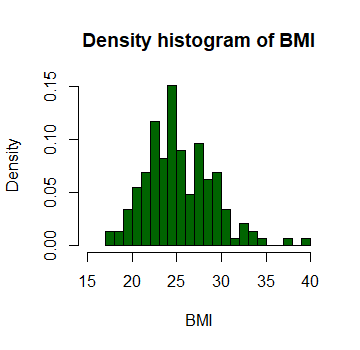
\includegraphics{root/Rplot1.png}
    \caption{Density histogram of BMI}
    \label{DensityHistEveryone}
\end{figure}
The empirical density is represented in the histogram above \ref{DensityHistEveryone}. From here it is easy to tell that the empirical distribution is not symmetrical and tends to be right-skewed. The majority of people have a BMI that lies in between 20 and 26, while there is a big range of variation since some values are close to 17 (severely underweight) and others to 40 (stage 2 obesity). Obviously the BMI can not be negative because that will imply either a negative weight or height. 

\subsection{c)}
\subsubsection{Males}
\begin{figure}[ht]
    \centering
    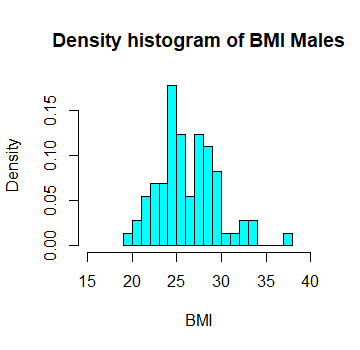
\includegraphics{root/Rplot2male.png}
    \caption{Density histogram of BMI Males}
    \label{DensityHistMale}
\end{figure}
The empirical density for males, represented in the histogram above \ref{DensityHistMale}, is more symmetrical than the one found for the whole data set \ref{DensityHistEveryone}. The most amount of people lie in between the BMI values of 23 and 28 and there are not so many discrepancy (it spreads from 19 to 33 BMI) except for an outlier that has 38 of BMI. There still are a lot of big variations (with some cases of obesity) but slightly reduced compared to the gender mixed one \ref{DensityHistEveryone}.
\newpage
\subsubsection{Females}
\begin{figure}[h!]
    \centering
    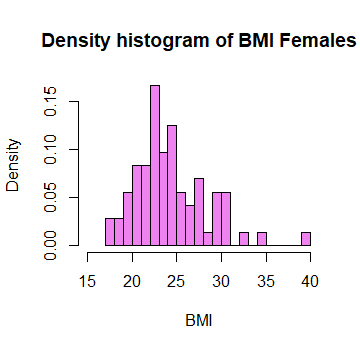
\includegraphics{root/Rplot2female.png}
    \caption{Density histogram of BMI Females}
    \label{DensityHistFemale}
\end{figure}

The empirical density for females is not symmetric at all, it is easy to notice that most people lie in the zone that goes from 20 to 25 BMI, which is a bit lower than males. The general discrepancy however is more amplified with BMI values that go form 17 to 40 (this last value is an outlier of type 2 obesity). In general it is possible to say that the female plot represents better the general density histogram \ref{DensityHistEveryone}, this is caused by the wider variation that can be observed in the females data.
\newpage

\subsection{d)}
\begin{figure}[h!]
    \centering
    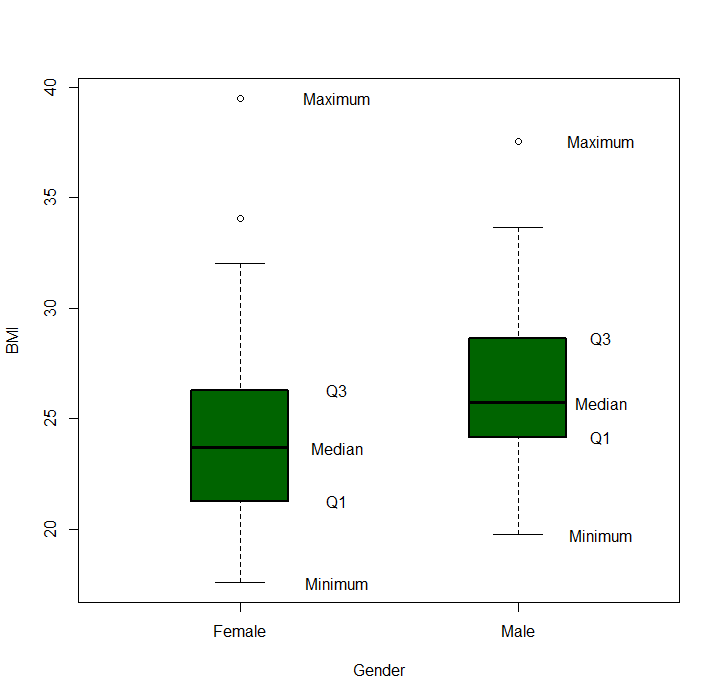
\includegraphics[scale=0.5]{root/Rplot3.png}
    \caption{Box-plot of BMI scores by gender}
    \label{Boxplot}
\end{figure}
The box plot \ref{Boxplot} helps us to point out where the quartiles, the median and the outliers are located in the distributions. It is not possible to say that the distributions are symmetrical (almost skewed); but they can become slightly symmetrical not considering the outliers. The difference between the two distribution is that the male one \ref{DensityHistMale} is more compact with less variation respect to the female one \ref{DensityHistFemale}. Talking about outliers it is possible to identify two of them for the females and one of them for the males (mentioned above).
\newpage

\subsection{e)}
Compared to the box plot \ref{Boxplot} using the table \ref{Table1} it is possible the see the standard deviation and the variance for the general distribution and for each subset.\\ 
\begin{table}[h!]
\begin{tabular}{|c||c|c|c|c|c|c|c|}
  \hline
\parbox{1.5cm}{\textbf{Variable} $BMI$} & \textbf{N. of obs.} & \parbox{1.5cm}{\textbf{Sample mean}} & \parbox{1.5cm}{\textbf{Sample var.}} & \parbox{1.5cm}{\textbf{Sample std. dev.}} & \parbox{1.5cm}{\textbf{Lower quart.}} & \textbf{Median} & \parbox{1.5cm}{\textbf{Upper quart}} \\ 
 \hline
  & $n$ & $(\overline{x})$ & $(s^2)$ & $(s)$ & $(Q_1)$ & $(Q_2)$ & $(Q_3)$ \\
  \hline
  \hline
Everyone & 145 & 25.25 & 14.69 & 3.83 & 22.59 & 24.69 & 27.64 \\ 
  \hline
  Women &  72 & 24.22 & 16.42 & 4.05 & 21.26 & 23.69 & 26.29 \\ 
    \hline
  Men &  73 & 26.27 & 11.07 & 3.33 & 24.15 & 25.73 & 28.63 \\ 
   \hline
\end{tabular}
\caption{Table with the required values for the data set}
\label{Table1}
\end{table}
